\section{Metameric Modulation}
\label{sec:metameric}
\graphicspath{{_MIMOColor/figures_mm/}}

\subsection{Human Eye And Color Perception}
\label{subsec:metamericEye}
The human eye is a sensory organ that enables humans to perceive electromagnetic radiation in a subset of the optical spectrum. \figurename{ \ref{figPhotopicCurve}} \cite{jai89a} shows the typical photopic relative luminous efficiency function of our visual system under moderate to higher levels of illumination. The retina in the eye contains sensory receptors called rods and cones. A normal human eye has three kinds of cones - short (S), medium (M) and long (L) based on the relative wavelengths that induce the peak response. Photons at different wavelengths are absorbed differently by the rods and the three sets of cones. \figurename{ \ref{figConeResp}} \cite{wan96a} shows the normalized absorbance of photons by rods and cones over a range of wavelengths. The peak responses of the cones are 420nm, 534nm and 564nm while that of the rods is 498nm. Cones are responsible for color vision. Let $S_{i}(\lambda)$ denote their spectral responses to stimulus over a range of wavelengths. Optical stimulus with a spectral power distribution (SPD) $C(\lambda)$ will induce optical sensation ${\alpha}_{S}, {\alpha}_{M}$ and ${\alpha}_{L}$ within the cones as described in (\ref{eqAlphaCones}).
\begin{equation}
	\label{eqAlphaCones}
	\alpha_{i} = \int\limits_{0}^{\infty} C(\lambda)S_{i}(\lambda)d\lambda
\end{equation}

\subsection{Metameric Modulation (MM)}
Grassmann's laws \cite{gra54a} of color matching develop the theory behind the psychovisual color space spanned by cones in the human eye, henceforth called the visual color space (VCS).  This space is a subspace  of the infinite dimensional universal color space (UCS), which contains all possible SPDs. This observation leads to another interpretation of (\ref{eqAlphaCones}) - the point $[{\alpha}_{S},{\alpha}_{M},{\alpha}_{L}]$ is a projection of a given SPD $C(\lambda)$ onto the VCS. Thus it is possible for multiple different SPDs to project onto the same point within the VCS and produce the same sensations, $[{\alpha}_{S},{\alpha}_{M},{\alpha}_{L}]$, in the human eye. These SPDs are sensed as the same color by the human eye and are called metamerically equivalent.

Light from three independent primary light sources can be mixed in varying amounts to generate arbitrary colors. We call this resulting color space the primary color space (PCS). The projection of the PCS onto the VCS is called the color gamut of the primaries.

The purpose of metameric modulation is to encode data in the visible spectrum while maintaining a constant ambient lighting state. To achieve this, at the transmitter, we use multiple primary sets each capable of generating its own color gamut. If we have $D$ sources and each primary set is rendered with $3$ primary elements, there are ${D\choose 3}$ possible primary sets. As the number of primary sets increases, the intersection of their color gamuts quickly approaches an empty set. However we select only $N$ of the possible primary sets so that the intersection of their color gamuts contain all of the desired lighting states. \figurename{ \ref{figCIEXYZMM}} shows an example for $D=4$ and $N=2$. The two sets of primaries, $[Blue, Cyan, Red]$ and $[Blue, Green, Red]$ have a significant overlap in their color gamuts. In this case they are capable of generating a set point with two different metameric SPDs. 

MM requires detection and discrimination of multiple wavelengths at the receiver. The necessary photodiodes must be designed such that when different primaries are activated to generate a desired ambient color, the receiver can detect which primary set is active while the lighting state appears the same to the human eye. The following derivation details how this can be achieved. 
\begin{figure}
	\centering
%		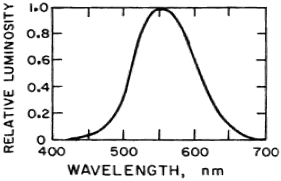
\includegraphics[width=3in]{PhotopicResponse.png}
    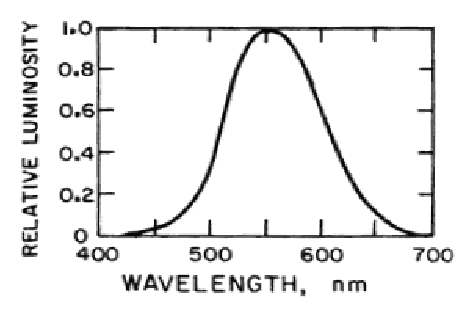
\includegraphics[width=3in]{PhotopicResponse.eps}
	\caption{Typical Photopic Relative Luminous Efficiency Function. Ref. \cite{jai89a}}
	\label{figPhotopicCurve}
\end{figure}

Initially consider three independent light sources that form one set of primaries. Let each $L_{k}(\lambda)$ be the normalized emission spectra of the $k^{th}$ of the three sources such that (\ref{eqNormEmm}) holds.
\begin{equation}
	\label{eqNormEmm}
	\int\limits_{0}^{\infty} L_{k}(\lambda)d\lambda = 1
\end{equation}
\begin{figure}
	\centering
%		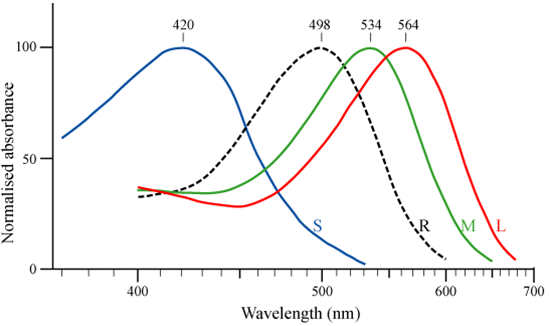
\includegraphics[width=4in]{ConeResponse.png}
    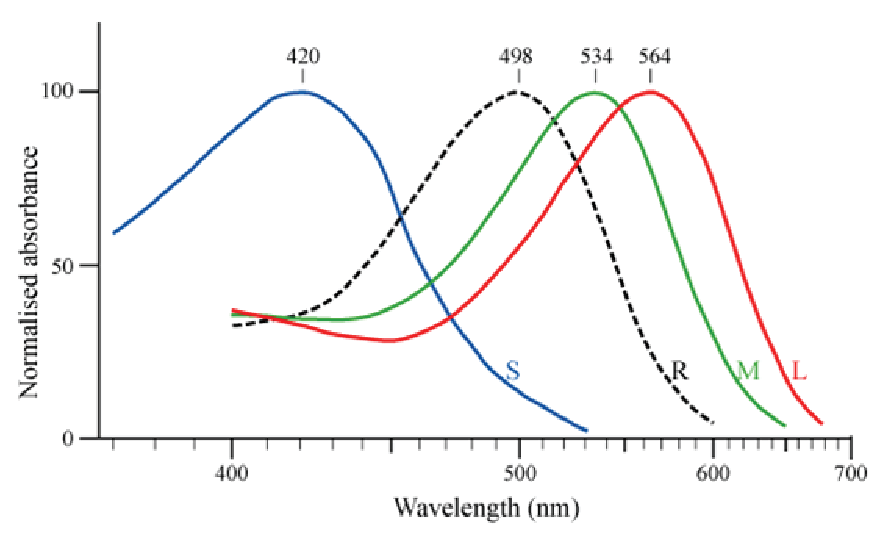
\includegraphics[width=4in]{ConeResponse.eps}
	\caption{Normalized Absorbance of Photons by Rods and Cones. Ref. \cite{wan96a}}
	\label{figConeResp}
\end{figure}

Let $\alpha_{i}^{k}$ (\ref{eqAlphaPrimaries}) be the spectral response induced by the $k^{th}$ primary on the $i^{th}$ class of cones.
\begin{equation}
	\label{eqAlphaPrimaries}
	\alpha_{i}^{k} = \int\limits_{0}^{\infty} L_{k}(\lambda)S_{i}(\lambda)d\lambda
\end{equation}

Let $C(\lambda)$ be the SPD of the ambient color that we wish to maintain. Let each $\beta_{k}$ be the amount of the corresponding $L_{k}(\lambda)$ needed to metamerically match $C(\lambda)$. Let $\alpha_{i}^{'}$ (\ref{eqAlphaPrime}) be the aggregate response evoked by the primaries on the $i^{th}$ class of cones. Grassmann's laws of color matching uphold the linearity property of color addition over a wide range of luminances. Our typical ambient illuminance levels lie well within this range of luminances.
\begin{equation}
	\label{eqAlphaPrime}
	\alpha_{i}^{'} = \sum\limits_{k=1}^{3} \beta_{k}\alpha_{i}^{k}
\end{equation}

The primaries must collectively evoke the same spectral responses in the human eye to match the color that is sensed due to $C(\lambda)$. Equating $\alpha_{i}$ in (\ref{eqAlphaCones}) with $\alpha_{i}^{'}$ in (\ref{eqAlphaPrime}) $\forall i$ leads to the color matching equation (\ref{eqColorMatch}). Solving for $\beta_{k}$ gives the relative amount of each primary that is needed to achieve a metamerical match with $C(\lambda)$.
\begin{equation}
	\label{eqColorMatch}
	\sum\limits_{k=1}^{3} \beta_{k}\int\limits_{0}^{\infty} L_{k}(\lambda)S_{i}(\lambda)d\lambda = \int\limits_{0}^{\infty} C(\lambda)S_{i}(\lambda)d\lambda
\end{equation}

Let $W(\lambda)$ be the SPD of the reference white against which the LEDs are calibrated. Let $w_{k}$ be the amount of $L_{k}(\lambda)$ needed to metamerically match $W(\lambda)$. Each tristimulus value, $t_{k}$, of each primary is defined in (\ref{eqTristimulus}). Varying $t_{k}$ for each primary changes the relative amount of the light output from each source that is mixed and thus changes color.
\begin{equation}
	\label{eqTristimulus}
	t_{k} = \beta_{k}/ w_{k}
\end{equation}

Now consider the case where we have $N$ sets of primaries each with $K$ (typically $K=3$) sources. Let the individual emission spectra of the $k^{th}$ source from the $n^{th}$ set of primaries be  $L_{k}^{n}(\lambda)$. Now, let us assume we have $P$ photodiodes  selected as mentioned above. Let the photodiode spectral responses be $S_{p}^{'}(\lambda)$. When light from all sources of the $n^{th}$ set of primaries is incident on the $p^{th}$ photodiode, its current output, $I_{p}^{n}$, is given by (\ref{eqPDCurrent}). 
\begin{equation}
	\label{eqPDCurrent}
	I_{p}^{n} = \sum\limits_{k=1}^{3} \beta_{k}\int\limits_{0}^{\infty} L_{k}^{n}(\lambda)S_{p}^{'}(\lambda)d\lambda
\end{equation}

\begin{figure}
	\centering
%		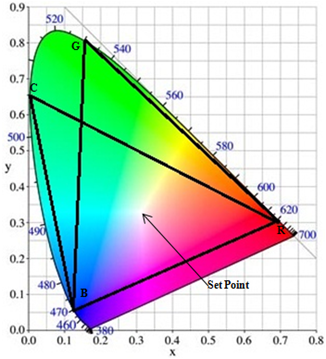
\includegraphics[width=2.5in]{CIE_XYZ_MM.png}
    
\includegraphics[width=2.5in]{CIE_XYZ_MM.eps}
	\caption{Example gamuts for metameric modulation with $N=2$, $D=4$ - B:Blue, C:Cyan, G:Green, R:Red overlayed on the CIE-XYZ chromaticity diagram}
	\label{figCIEXYZMM}
\end{figure}

\begin{table*}[b]
	\centering
		\begin{tabular}{|c|c|}
		\hline
		{Primary Set Index} & {Symbol}\\
		\hline
		1 & 00\\
		2 & 01\\
		3 & 10\\
		4 & 11\\
		\hline
		\end{tabular}
	\caption{Metameric Channel Symbol Assignment}
	\label{tblMMSymbol}
\end{table*}

For a given color, the response matrix $R_{g}$ is given by (\ref{eqRespMatrix}). It is possible to design a system where every column of matrix $R_{g}$ would be distinct. This system design is beyond the scope of this paper. By comparing the output of the photodiodes with the columns of $R_{g}$, the system can then detect which set of primaries is currently active.
\begin{equation}
	\label{eqRespMatrix}
R_{g} = \left( \begin{array}{ccc}
I_{1}^{1}&\cdots&I_{1}^{N}\\
\vdots&\ddots&\vdots\\
I_{P}^{1}&\cdots&I_{P}^{N}
\end{array} \right)
\end{equation}
The desired ambient lighting state can be specified by a point in the standard CIE-XYZ coordinate system for standard observer. For this given set point, the constellation diagram should be a set of unique points in the RCS which corresponds to the set point for each primary set. Table \ref{tblMMSymbol} shows symbol assignment for $N=4$. Well known color space transforms can then be applied to specify the desired color within the $N$ individual coordinate systems for each individual primary set. Let $t_{k}^{n}$ be the tristimulus value of the $k^{th}$ primary of the $n^{th}$ primary set. These primary sets can now generate distinct but metamerically equivalent SPDs. Switching between the different primary sets generates the data stream.

\begin{figure}[t]
	\centering
%		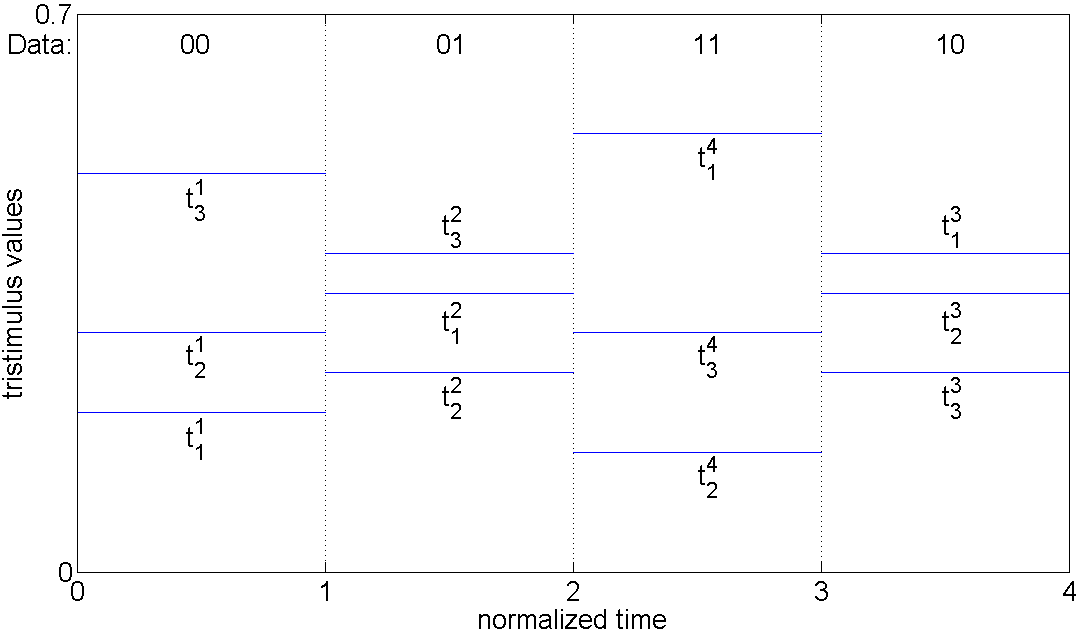
\includegraphics[width=5in]{MM_time.png}
    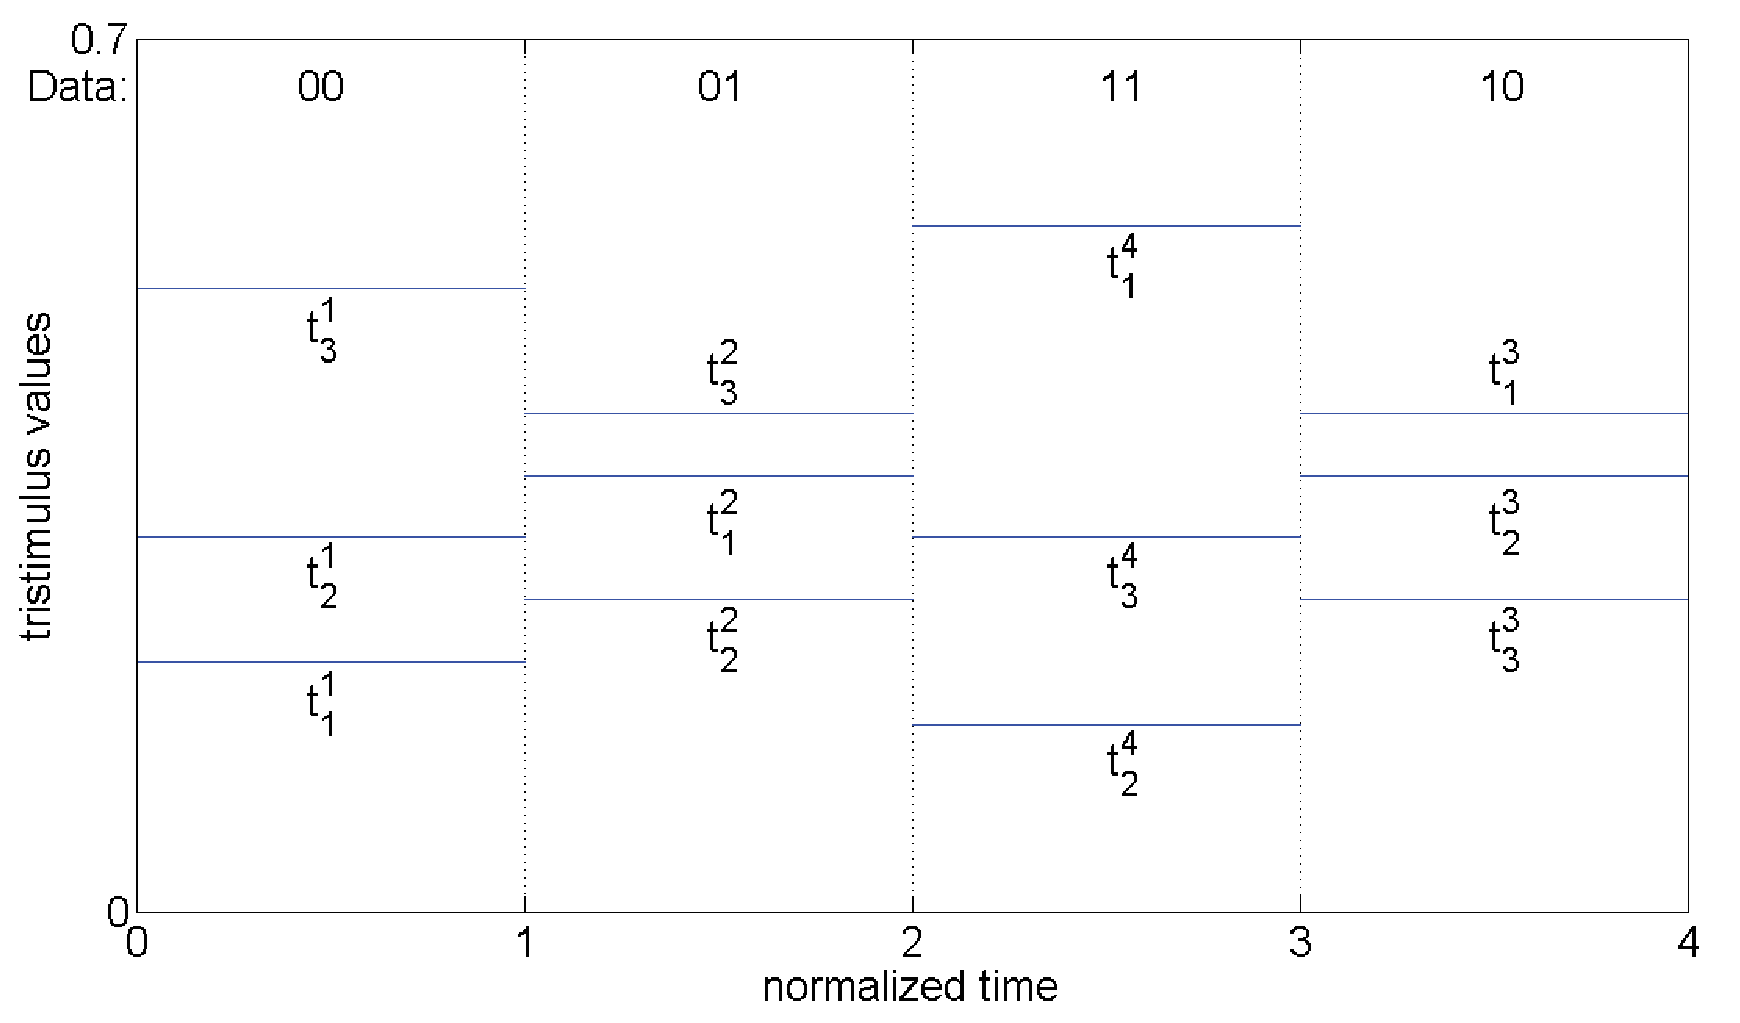
\includegraphics[width=5in]{MM_time.eps}
	\caption{MM example timing diagram}
	\label{figMMex}
\end{figure}

\figurename{ \ref{figMMex}} illustrates MM using these primary sets to transmit a part of a data stream $(00011110_{2})$. This is accomplished by switching primaries in the order 1-2-4-3. This order can then be detected by analyzing the photodiode outputs and data can be decoded. The embedded MM modulation is invisible to humans due to metamerism.


